\section{Méthodes numériques de résolution d'équations différentielles}
Dans cette partie, nous montrons les différentes méthodes de résolution numériques des équations différentielles afin d'en approximer les solutions.\\

\subsection{Algorithmes de résolution}

\textbf{Algorithme meth\_n\_step($y_0$, $t_0$, $N$, $f$, $step\_method$)}\\
Considérons l'intervalle $[t_0, t_f]$ représentant l'intervalle de temps durant lequel nous approximons la solution. Le but de cet algorithme consiste en la résolution de l'équation différentielle par calculs successifs des points $y_n$ au moment $t_n$. Pour ce faire, nous avons implémenté 4 méthodes de résolution différentes (Euler, Point milieu, Heun et Runge-Kutta d'ordre 4). Ces fonctions se présentent sous la forme \texttt{step\_<used\_method>($y_n$, $t_n$, $h$, $f$)}, avec $h$ le pas, et $f$ la fonction solution de $f(y,t) = y'(t)$. Le calcul de l'ensemble des points $y_0,...y_f$ correspondant à $N$ divisions de l'intervalle de départ, peuvent être calculés.\\

\textbf{Algorithme meth\_epsilon($y_0$, $t_0$, $N$, $f$, $step\_method$)}\\
Cet algorithme a pour but d'approximer une solution de l'équation différentielle avec une précision $\varepsilon$. Pour cela, calculons une première solution par le biais de l'algorithme précédent. Ensuite, nous nous approchons de la précision $\varepsilon$ grâce à une \textbf{boucle}. Cette boucle double $N$, et double la précision du pas $h$ à chaque itération. Ces nouvelles valeurs sont ensuite utilisées avec l'algorithme précédent pour calculer la nouvelle norme. Cette boucle est répétée tant que la précision $\varepsilon$ et le nombre maximum d'itérations ne sont pas atteints.

Cette méthode a pour avantage de rectifier la courbe de la pente à chaque itération, s'approchant de fait toujours plus de la solution exacte. Toutefois, toutes les méthodes ne se valent pas, par conséquent le nombre de points nécessaires pour approximer une solution avec une précision $\varepsilon$ fluctue.

\subsection{Tests des implémentations}
Afin de tester nos implémentations, nous avons tracer les solutions pour les deux équations différentielles \ref{eq:dim1} et \ref{eq:dim2} suivantes.

\begin{equation}
    \left\{
    \begin{array}{ll}
        y(0) &= 1 \\
        y'(t) &= \frac{y(t)}{1 + t^2}
    \end{array}
\right.
\label{eq:dim1}
\end{equation}

\begin{equation}
    \left\{
    \begin{array}{ll}
        y(0) &= \begin{bmatrix}
                    0 \\
                    1
                \end{bmatrix} \\
        y'(t) &= \begin{bmatrix}
                    -y_2(t) \\
                    y_1(t)
                \end{bmatrix} \\
    \end{array}
\right.
\label{eq:dim2}
\end{equation}

\begin{minipage}[c]{.46\linewidth}
    \centering
    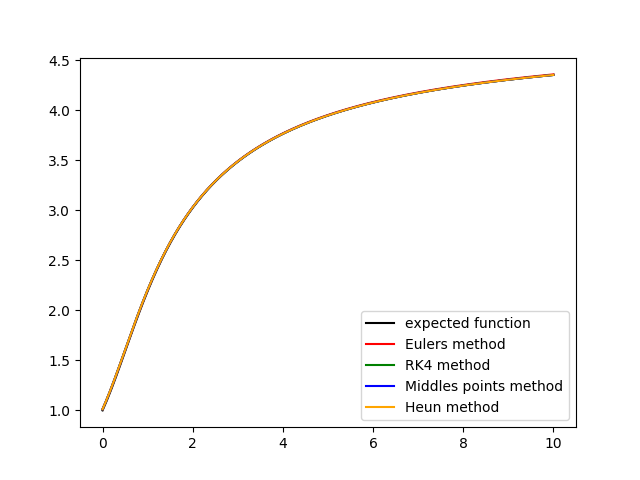
\includegraphics[scale=0.5]{images/dim1.png}
    \captionsetup{type=figure}\caption{Courbes solution de l'équation différentielle \ref{eq:dim1} pour $\varepsilon = 10^{-2}$ (solution exacte : $\exp\arctan(x)$)}
    \label{fig:dim1}
\end{minipage}
\hfill%
\begin{minipage}[c]{.46\linewidth}
    \centering
    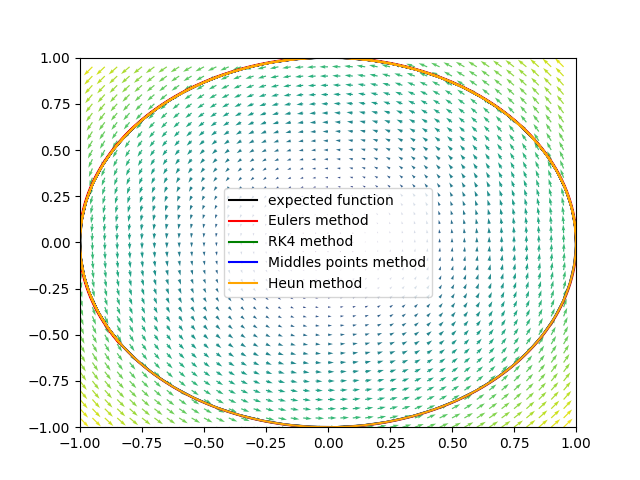
\includegraphics[scale=0.5]{images/dim2.png}
    \captionsetup{type=figure}\caption{Champs de tangentes et courbes solution de l'équation différentielle \ref{eq:dim2} pour $\varepsilon = 10^{-2}$
    (solution exacte : $[cos(x), sin(x)]$)}
    \label{fig:dim2}
\end{minipage}
\vspace{4.00mm}

On remarque nettement sur les deux figures \ref{eq:dim1}et \ref{eq:dim2} précédentes que toutes les méthodes convergent précisément vers la solution souhaitée dès lors que le $\varepsilon$ choisi est suffisamment précis.
De plus, on aperçoit sur la figure \ref{fig:dim2} que le champs de tangentes est suivi par l'approximation de nos solutions. Par conséquent, les méthodes semble correctement implémentées.

Néanmoins, nous avons rencontré des erreurs concernant les dimensions associées aux fonctions des équations différentielles. En effet, le code associé à l'algorithme \textbf{meth\_n\_step($y_0$, $t_0$, $N$, $f$, $step\_method$)} devait être implémenté de telle sorte à accepter ces différentes dimensions. De plus, comme nous l'avons évoqué précédemment pour l'algorithme \textbf{meth\_epsilon($y_0$, $t_0$, $N$, $f$, $step\_method$)} il était nécessaire d'ajouter une condition d'arrêt concernant le nombre d'itérations effectuées. En effet, son absence pouvait entraîner des boucles infinies dans le cas d'une non convergence.